\chapter{Calculations and results}

The hardest task in doing the calculations was to write out the matrix
elements, to be read by another program that performs the coupled
cluster calculations.% As we wanted to make as good a calculation as possible we
%tried to make the model space as huge as possible.% We soon realized that it
%would take to much time.\\
\\
When operating in a plane wave basis we have both mesh points for the numerical
integration and the orbital angular momentum number $l$  to consider because of
the partial wave expansion. The idea was to fix the maximum value of $l$ to six, and
number of mesh points to 12. However it seemed that the maximum orbital angular
momentum number had to be lowered to finish the thesis in time.\\% Of course the
%precision would be much better with both increasing the orbital angular
%momentum number and mesh points and it is assumed that the values predicted would have
%improved.\\
\\
As we are doing the calculations with just two-body forces, and in a plane wave
basis, the Hamiltonian is composed of the kinetic energy  and a
two-body interaction as seen in the Hamiltonian
\begin{equation*}
		\begin{split}
				&H=\sum_{i=0}^A\frac{1}{2m}\bra{i}k^2\ket{i}a^\dagger_ia_i + \frac{1}{2}\sum_{ijkl}\bra{ij}v\ket{kl}a^\dagger_ia^\dagger_ja_la_k.
		\end{split}
\end{equation*}
When we integrate over the momentum we will be left with an undefined volume term
$\Omega$, to get a definite answer we divide with the number of particles. 
Technically this is done by dividing each energy term by the volume, $\Omega$, and 
the density, $\rho$, defined in Eq \eqref{eq:density} to get the expression
\begin{equation*}
		\begin{split}
			&	 \sum_{jt_z} (2j+1)\int _0^{k_f}\frac{k^4}{2\pi^2}dk\frac{1}{2m_N\rho}+\\
			&	\sum_{\substack{j_1l_l1t_{z_1}\\j_2l_2t_{z_2}}}\sum_{\substack{j_3l_3t_{z_3}\\j_4l_4t_{z_4}}}(2J+1)\int \frac{d^3k_1 d^3k_2 d^3k_3 d^3k_4}{(2\pi)^{12}\rho}\bra{j_1l_1k_1t_{z_1}j_2l_2k_2t_{z_2}JT_z}v
				\ket{j_3l_3k_3t_{z_3}j_4l_4k_4t_{z_4}JT_z}.
		\end{split}
\end{equation*}
In a numerical calculation the integrals over $k$ become sums, 
\begin{equation*}
		\int f(k)k^2dk \rightarrow \sum_i^N f(k_i)k^2_i\omega _i
\end{equation*}
In performing the integrals numerically Gaussian quadrature was used, for details see \cite{compphys-mhjensen}.\\
\\
The nuclear interaction model used is N$^3$LO \cite{entem-2003-68} with cutoff, 
$\Lambda=500$ MeV. We
renormalized the $N^3LO$ potential with $V_{low-k}$, the cutoff,  $\lambda$, 
used was 2.1 $\mbox{fm}^{-1}$, 2.2 fm$^{-1}$ and 2.5 fm$^{-1}$.\\
\\
%%sjekk
Most calculations on nuclear matter have been done with a
perturbational approach by renormalizing the potential with for example  $V_{low-k}$ as a
renormalization scheme. The Brueckner $G$-matrix approach is also a often used method to do computations on nuclear matter. It is a way to circumvent
the strictly unperturbative part of the nuclear interactions, it is briefly described
in appendix \ref{bgm}.  
\\
\section{The programs}

Two separate programs were used, one which calculates the interaction elements in
the laboratory frame and then the other program that performs the coupled cluster
computations. As said above the hardest task was to compute the interactions,
it was really slow because of the bracket transformations.  In order to improve
the efficiency it had to be parallelized. It was not so difficult to parallellize the program since one interaction element does not depend on another element. 
The computation of interaction elements were 
spread evenly to different processes.  
The pseudo-code below shows how a for-loop was parallelized.
\begin{algorithm}
\begin{algorithmic}
		\FOR{$i$= iam+1, n, numprocs}
         \STATE   some code
        \ENDFOR
\end{algorithmic}
\end{algorithm}\\
Complications
arose when the interaction elements were written to the file to be read by the coupled cluster
program.  The easiest way was to let each process write their matrix elements
to their own file and then concatenate the files to one. This is a rather fast
process but it generates a lots of files and is not always approved by the
cluster administrators and some clusters will only let the master node write to
file.  What was done was to let each process store their interaction elements in
an array which was sent to the master node which writes them to a file. This
is a rather tedious and slow process and it is not recommended.\\
\\
A better method
would be to use the MPI I/O functions, which let the processes write to the
same file. The complications which made us avoid the MPI I/O method was that we
needed to know both the total file size and the size each processes write.
Because of the bracket transformations it was difficult to 
know how much each process would
write. We came to the conclusion that if we give the processes a too huge size
of the file than necessary, it could generate blank lines, which may get problematic when reading it. Another MPI tool to use is NETCDF4/HDF5, however with this it was difficult to write the matrix elements in the form the coupled cluster
program demands.\\
\\
The coupled cluster program used, was originally written in a harmonic oscillator basis. 
Some minor changes in how the program reads the interactions, had to be performed to make the coupled cluster program work in a plane wave basis as well. 
For not change the program too much the matrix elements to be read were already multiplied with the mesh points and weights for the integrations
\begin{equation*}
		\begin{split}
             &\bra{l_1j_1k_2l_2k_2JT_z}v\ket{l_3j_3k_3l_4j_4k_4JT_z}\\
             & \rightarrow \bra{l_1j_1k_1l_2j_2k_2JT_z}v\ket{l_3j_3k_3l_4j_4k_4JT_z}k_1k_2k_3k_4\sqrt{w_1w_2w_3w_4}.
        \end{split}
\end{equation*}
Then the only thing needed was to multiply with the factor $1/(2\pi)^2$  for
each integration variable and keep in mind that nothing should be divided by
the weights and mesh points when solving for the cluster amplitudes. 

\clearpage


\section{Results and conclusion}

The aim of the thesis was to calculate the binding energy of symmetric nuclear
matter  with the coupled cluster method. As this was done in a plane wave basis, we had to do an
integration over momentum, $k$, in the region where $k\in[0,\infty]$.
Numerically this is accomplished by a tangential mapping. As the
renormalization scheme V$_{low-k}$ was used, the problem is projected to
a smaller space by defining $k\in[0,\lambda]$, where $\lambda$ usually ranges from 2
fm$^{-1}$ to 3 fm$^{-1}$. The tangential projection procedure was omitted since
the meshpoints were projected onto the new interval $k\in[0,\lambda]$.\\
\\
In chapter \ref{ch:coupled} we saw that when doing coupled cluster calculation
we have to make a distinction between particles and holes. In chapter
\ref{chapsecondq} we defined holes as particles inside the Fermi sphere and
particles to be outside. The radius of the Fermi sphere was set to be $k_f$
where $k_f$ ranges from 1.2 fm$^{-1}$ to 1.9 fm$^{-1}$. All single-particle
states with a momentum below or equal $k_f$ are to be holes and those with a
momentum greater than $k_f$ were defined as particles.\\
\\
In Figs.~\ref{fig:hf21}-\ref{fig:hf23} we present the first-order energies for orbital angular momentum, $l$, values
truncated at four and six.  The saturation density remains more or less constant
for both $l$-values at 1.75 fm$^{-1}$, which is greater than the experimental
value at 1.42 fm$^{-1}$. The binding energy, approximately $3$MeV, are way too low for orbital angular momentum
truncated at 4, compared to the experimental value, 16 MeV. For $\lambda=2.5$
fm$^{-1}$ the first order approximation failed to give a minimum.
An interesting observation is that the
cutoff  $\lambda=2.1$ fm$^{-1}$ gives a higher binding energy (lower minimum) than the cutoff
on 2.2 fm$^{-1}$. This because the  interaction elements with lower $\lambda$
have higher absolute values. This will of course have an effect on the coupled cluster
computations as well. It is believed that three-body forces may correct for the dependency on the cutoff.\\
\\
The first order calculations with angular momentum truncated at 6 and 
$\lambda=2.2$ almost reproduces the experimental binding energy, but with a 
higher cutoff the interaction elements get smaller and fails to reproduce the 
experimental binding energy. Coupled cluster computation on $l=6$ was not 
completed it was time consuming and it required too much memory.\\
\\
In the case of pure neutron matter the equation of state is almost 
constant in the cutoff, which can be seen in Figs.~\ref{fig:first_neutron_l4} and \ref{fig:ccm_net_4_21}.\\
\\
In Figs \ref{fig:ccm_nucl_4_21} and \ref{fig:ccm_net_4_21} we present coupled cluster calculations on symmetric nuclear matter and pure neutron matter respectively.
We see that it is almost identical to the first-order energies.% for first order
%
\begin{table}
		\centering
		\begin{tabular}{|c|c|c|c|c|c|}
				\hline
				\multicolumn{3}{|c|}{$\lambda=2.1$ fm$^{-1}$}& \multicolumn{3}{c|}{$l_{\mbox{max}}=4$ }\\
				\hline
				$k_f$ & Total energy & $\sum_{ai}f_{ai}t^a_i$ & $\sum_{abij}v_{abij}t^a_it^b_j$ & $\sum_{abij}v_{abij}t^{ab}_{ij}$ & Total correction\\
				\hline
				1.2 & 3.787507 & -0.030488 & -0.000117 & -0.058656 & -0.089261  \\
				\hline
				1.4 & 3.82199 &  -0.030239 & -0.000889 & -0.145316 & -0.175644\\
				\hline
				1.6 & -2.071725 & -0.057642 & -0.000140 & -0.113498 & -0.171280 \\
				\hline
				1.8 & -4.307874 & -0.117001 & -0.000423 & -0.058656 & 0.176080 \\
				\hline
				1.9 & 0.215606 & -0.05693 & -0.000129 & -0.032594 & -0.089660 \\
				\hline
		%		\hline
				\multicolumn{3}{|c|}{$\lambda=2.2$ fm$^{-1}$}& \multicolumn{3}{c|}{$l_{\mbox{max}}=4$ }\\
				\hline
				$k_f$ & Total energy & $\sum_{ai}f_{ai}t^a_i$ & $\sum_{abij}v_{abij}t^a_it^b_j$ & $\sum_{abij}v_{abij}t^{ab}_{ij}$ & Total correction\\
				\hline
				1.2 & 2.856008 & -0.025748 & -0.000100 & -0.153787 & -0.179635\\
				\hline
				1.4 & 3.664643 & -0.026888 & -0.000006 & -0.175784 & -0.202737\\
			    \hline
				1.6 & 1.429075 & -0.075102 & -0.000432 & -0.184876 & -0.260410\\
				\hline
				1.7 &-4.663540 & -0.186931 & -0.002106 & -0.169220 & -0.358257\\
				\hline
				\multicolumn{3}{|c|}{$\lambda=2.5$ fm$^{-1}$}& \multicolumn{3}{c|}{$l_{\mbox{max}}=4$ }\\
				\hline
				1.4 & 6.426474 & 0.001282 & 0.000037 & -0.322986 & -0.321667\\
				\hline
			%	\multicolumn{3}{|c|}{$\lambda=3.0$ fm$^{-1}$}& \multicolumn{3}{c|}{$l_{\mbox{max}}=4$ }\\
			%	\hline
			%	\multicolumn{3}{|c|}{$\lambda=2.2$ fm$^{-1}$}& \multicolumn{3}{c|}{$l_{\mbox{max}}=6$ }\\
			%	\hline
		\end{tabular}
		\caption{Energies and correction to the first order energy for different values of $\lambda$ and $k_f$. All energies are in MeV}
		\label{tab:korreksjoner}
\end{table}
%it seems that the cluster amplitudes are almost zero, meaning that the state $\Psi$ is almost identical to the state $\Phi_0$. 
\begin{figure}[htpb]
		% GNUPLOT: LaTeX picture with Postscript
\begingroup
  \makeatletter
  \providecommand\color[2][]{%
    \GenericError{(gnuplot) \space\space\space\@spaces}{%
      Package color not loaded in conjunction with
      terminal option `colourtext'%
    }{See the gnuplot documentation for explanation.%
    }{Either use 'blacktext' in gnuplot or load the package
      color.sty in LaTeX.}%
    \renewcommand\color[2][]{}%
  }%
  \providecommand\includegraphics[2][]{%
    \GenericError{(gnuplot) \space\space\space\@spaces}{%
      Package graphicx or graphics not loaded%
    }{See the gnuplot documentation for explanation.%
    }{The gnuplot epslatex terminal needs graphicx.sty or graphics.sty.}%
    \renewcommand\includegraphics[2][]{}%
  }%
  \providecommand\rotatebox[2]{#2}%
  \@ifundefined{ifGPcolor}{%
    \newif\ifGPcolor
    \GPcolortrue
  }{}%
  \@ifundefined{ifGPblacktext}{%
    \newif\ifGPblacktext
    \GPblacktexttrue
  }{}%
  % define a \g@addto@macro without @ in the name:
  \let\gplgaddtomacro\g@addto@macro
  % define empty templates for all commands taking text:
  \gdef\gplbacktext{}%
  \gdef\gplfronttext{}%
  \makeatother
  \ifGPblacktext
    % no textcolor at all
    \def\colorrgb#1{}%
    \def\colorgray#1{}%
  \else
    % gray or color?
    \ifGPcolor
      \def\colorrgb#1{\color[rgb]{#1}}%
      \def\colorgray#1{\color[gray]{#1}}%
      \expandafter\def\csname LTw\endcsname{\color{white}}%
      \expandafter\def\csname LTb\endcsname{\color{black}}%
      \expandafter\def\csname LTa\endcsname{\color{black}}%
      \expandafter\def\csname LT0\endcsname{\color[rgb]{1,0,0}}%
      \expandafter\def\csname LT1\endcsname{\color[rgb]{0,1,0}}%
      \expandafter\def\csname LT2\endcsname{\color[rgb]{0,0,1}}%
      \expandafter\def\csname LT3\endcsname{\color[rgb]{1,0,1}}%
      \expandafter\def\csname LT4\endcsname{\color[rgb]{0,1,1}}%
      \expandafter\def\csname LT5\endcsname{\color[rgb]{1,1,0}}%
      \expandafter\def\csname LT6\endcsname{\color[rgb]{0,0,0}}%
      \expandafter\def\csname LT7\endcsname{\color[rgb]{1,0.3,0}}%
      \expandafter\def\csname LT8\endcsname{\color[rgb]{0.5,0.5,0.5}}%
    \else
      % gray
      \def\colorrgb#1{\color{black}}%
      \def\colorgray#1{\color[gray]{#1}}%
      \expandafter\def\csname LTw\endcsname{\color{white}}%
      \expandafter\def\csname LTb\endcsname{\color{black}}%
      \expandafter\def\csname LTa\endcsname{\color{black}}%
      \expandafter\def\csname LT0\endcsname{\color{black}}%
      \expandafter\def\csname LT1\endcsname{\color{black}}%
      \expandafter\def\csname LT2\endcsname{\color{black}}%
      \expandafter\def\csname LT3\endcsname{\color{black}}%
      \expandafter\def\csname LT4\endcsname{\color{black}}%
      \expandafter\def\csname LT5\endcsname{\color{black}}%
      \expandafter\def\csname LT6\endcsname{\color{black}}%
      \expandafter\def\csname LT7\endcsname{\color{black}}%
      \expandafter\def\csname LT8\endcsname{\color{black}}%
    \fi
  \fi
  \setlength{\unitlength}{0.0500bp}%
  \begin{picture}(7200.00,5040.00)%
    \gplgaddtomacro\gplbacktext{%
      \csname LTb\endcsname%
      \put(990,660){\makebox(0,0)[r]{\strut{}$-6$}}%
      \put(990,1280){\makebox(0,0)[r]{\strut{}$-4$}}%
      \put(990,1900){\makebox(0,0)[r]{\strut{}$-2$}}%
      \put(990,2520){\makebox(0,0)[r]{\strut{}$0$}}%
      \put(990,3140){\makebox(0,0)[r]{\strut{}$2$}}%
      \put(990,3760){\makebox(0,0)[r]{\strut{}$4$}}%
      \put(990,4380){\makebox(0,0)[r]{\strut{}$6$}}%
      \put(1122,440){\makebox(0,0){\strut{}$1.2$}}%
      \put(1835,440){\makebox(0,0){\strut{}$1.3$}}%
      \put(2548,440){\makebox(0,0){\strut{}$1.4$}}%
      \put(3261,440){\makebox(0,0){\strut{}$1.5$}}%
      \put(3974,440){\makebox(0,0){\strut{}$1.6$}}%
      \put(4687,440){\makebox(0,0){\strut{}$1.7$}}%
      \put(5400,440){\makebox(0,0){\strut{}$1.8$}}%
      \put(6113,440){\makebox(0,0){\strut{}$1.9$}}%
      \put(6826,440){\makebox(0,0){\strut{}$2$}}%
      \put(220,2520){\rotatebox{90}{\makebox(0,0){\strut{}E/A [MeV]}}}%
      \put(3974,110){\makebox(0,0){\strut{}$k_f$}}%
      \put(3974,5110){\makebox(0,0){\strut{}First order energies for symmetric nuclear matter $l=4$.}}%
    }%
    \gplgaddtomacro\gplfronttext{%
      \csname LTb\endcsname%
      \put(6169,4607){\makebox(0,0)[r]{\strut{}$\lambda=2.1$ fm$^{-1}$}}%
      \csname LTb\endcsname%
      \put(6169,4387){\makebox(0,0)[r]{\strut{}$\lambda=2.2$ fm$^{-1}$}}%
      \csname LTb\endcsname%
      \put(6169,4167){\makebox(0,0)[r]{\strut{}$\lambda=2.5$ fm$^{-1}$}}%
    }%
    \gplbacktext
    \put(0,0){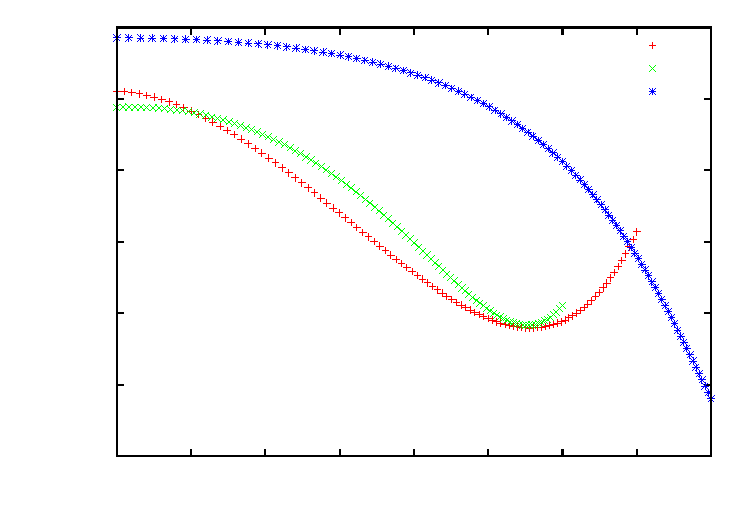
\includegraphics{symmetric_hfl4_2_1}}%
    \gplfronttext
  \end{picture}%
\endgroup

		\caption{First-order energy for orbital angular momentum truncated at 4, and a cutoff  $\lambda=2.1$fm$^{-1}$, $\lambda=2.2$fm$^{-1}$ and $\lambda=2.5$ fm$^{-1}$.}
		\label{fig:hf21}
\end{figure}
%\begin{figure}[htpb]
%		% GNUPLOT: LaTeX picture with Postscript
\begingroup
  \makeatletter
  \providecommand\color[2][]{%
    \GenericError{(gnuplot) \space\space\space\@spaces}{%
      Package color not loaded in conjunction with
      terminal option `colourtext'%
    }{See the gnuplot documentation for explanation.%
    }{Either use 'blacktext' in gnuplot or load the package
      color.sty in LaTeX.}%
    \renewcommand\color[2][]{}%
  }%
  \providecommand\includegraphics[2][]{%
    \GenericError{(gnuplot) \space\space\space\@spaces}{%
      Package graphicx or graphics not loaded%
    }{See the gnuplot documentation for explanation.%
    }{The gnuplot epslatex terminal needs graphicx.sty or graphics.sty.}%
    \renewcommand\includegraphics[2][]{}%
  }%
  \providecommand\rotatebox[2]{#2}%
  \@ifundefined{ifGPcolor}{%
    \newif\ifGPcolor
    \GPcolortrue
  }{}%
  \@ifundefined{ifGPblacktext}{%
    \newif\ifGPblacktext
    \GPblacktexttrue
  }{}%
  % define a \g@addto@macro without @ in the name:
  \let\gplgaddtomacro\g@addto@macro
  % define empty templates for all commands taking text:
  \gdef\gplbacktext{}%
  \gdef\gplfronttext{}%
  \makeatother
  \ifGPblacktext
    % no textcolor at all
    \def\colorrgb#1{}%
    \def\colorgray#1{}%
  \else
    % gray or color?
    \ifGPcolor
      \def\colorrgb#1{\color[rgb]{#1}}%
      \def\colorgray#1{\color[gray]{#1}}%
      \expandafter\def\csname LTw\endcsname{\color{white}}%
      \expandafter\def\csname LTb\endcsname{\color{black}}%
      \expandafter\def\csname LTa\endcsname{\color{black}}%
      \expandafter\def\csname LT0\endcsname{\color[rgb]{1,0,0}}%
      \expandafter\def\csname LT1\endcsname{\color[rgb]{0,1,0}}%
      \expandafter\def\csname LT2\endcsname{\color[rgb]{0,0,1}}%
      \expandafter\def\csname LT3\endcsname{\color[rgb]{1,0,1}}%
      \expandafter\def\csname LT4\endcsname{\color[rgb]{0,1,1}}%
      \expandafter\def\csname LT5\endcsname{\color[rgb]{1,1,0}}%
      \expandafter\def\csname LT6\endcsname{\color[rgb]{0,0,0}}%
      \expandafter\def\csname LT7\endcsname{\color[rgb]{1,0.3,0}}%
      \expandafter\def\csname LT8\endcsname{\color[rgb]{0.5,0.5,0.5}}%
    \else
      % gray
      \def\colorrgb#1{\color{black}}%
      \def\colorgray#1{\color[gray]{#1}}%
      \expandafter\def\csname LTw\endcsname{\color{white}}%
      \expandafter\def\csname LTb\endcsname{\color{black}}%
      \expandafter\def\csname LTa\endcsname{\color{black}}%
      \expandafter\def\csname LT0\endcsname{\color{black}}%
      \expandafter\def\csname LT1\endcsname{\color{black}}%
      \expandafter\def\csname LT2\endcsname{\color{black}}%
      \expandafter\def\csname LT3\endcsname{\color{black}}%
      \expandafter\def\csname LT4\endcsname{\color{black}}%
      \expandafter\def\csname LT5\endcsname{\color{black}}%
      \expandafter\def\csname LT6\endcsname{\color{black}}%
      \expandafter\def\csname LT7\endcsname{\color{black}}%
      \expandafter\def\csname LT8\endcsname{\color{black}}%
    \fi
  \fi
  \setlength{\unitlength}{0.0500bp}%
  \begin{picture}(7200.00,5040.00)%
    \gplgaddtomacro\gplbacktext{%
      \csname LTb\endcsname%
      \put(990,660){\makebox(0,0)[r]{\strut{}$-5$}}%
      \put(990,1117){\makebox(0,0)[r]{\strut{}$-4$}}%
      \put(990,1575){\makebox(0,0)[r]{\strut{}$-3$}}%
      \put(990,2032){\makebox(0,0)[r]{\strut{}$-2$}}%
      \put(990,2489){\makebox(0,0)[r]{\strut{}$-1$}}%
      \put(990,2947){\makebox(0,0)[r]{\strut{}$0$}}%
      \put(990,3404){\makebox(0,0)[r]{\strut{}$1$}}%
      \put(990,3861){\makebox(0,0)[r]{\strut{}$2$}}%
      \put(990,4319){\makebox(0,0)[r]{\strut{}$3$}}%
      \put(990,4776){\makebox(0,0)[r]{\strut{}$4$}}%
      \put(1122,440){\makebox(0,0){\strut{}$1.2$}}%
      \put(1835,440){\makebox(0,0){\strut{}$1.3$}}%
      \put(2548,440){\makebox(0,0){\strut{}$1.4$}}%
      \put(3261,440){\makebox(0,0){\strut{}$1.5$}}%
      \put(3974,440){\makebox(0,0){\strut{}$1.6$}}%
      \put(4687,440){\makebox(0,0){\strut{}$1.7$}}%
      \put(5400,440){\makebox(0,0){\strut{}$1.8$}}%
      \put(6113,440){\makebox(0,0){\strut{}$1.9$}}%
      \put(6826,440){\makebox(0,0){\strut{}$2$}}%
      \put(220,2718){\rotatebox{90}{\makebox(0,0){\strut{}E/A [MeV]}}}%
      \put(3974,110){\makebox(0,0){\strut{}$k_f$}}%
    }%
    \gplgaddtomacro\gplfronttext{%
      \csname LTb\endcsname%
      \put(5839,4603){\makebox(0,0)[r]{\strut{}E/A Hartree-Fock l=4 $\lambda$=2.2 fm$^{-1}$}}%
    }%
    \gplbacktext
    \put(0,0){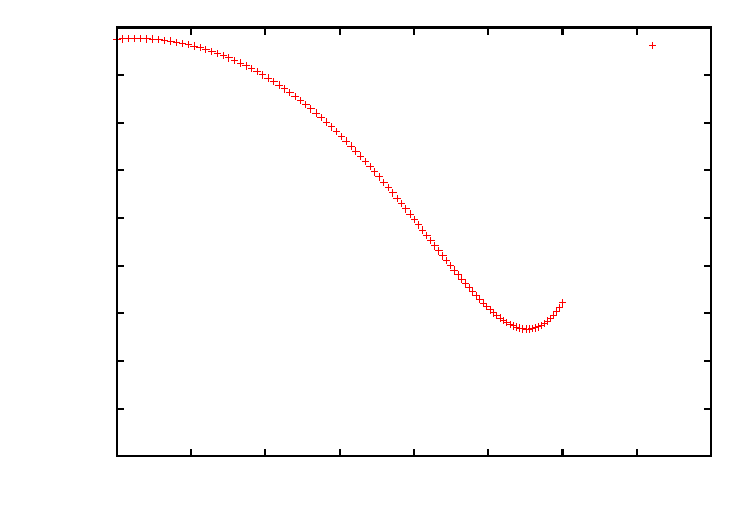
\includegraphics{symmetric_hfl4_2_2}}%
    \gplfronttext
  \end{picture}%
\endgroup

%		\caption{Hartree-Fock energy for orbital momentum truncated at 4, and a cutoff $\lambda=2.2$.}
%		\label{fig:hf22}
%\end{figure}
\begin{figure}[htpb]
		% GNUPLOT: LaTeX picture with Postscript
\begingroup
  \makeatletter
  \providecommand\color[2][]{%
    \GenericError{(gnuplot) \space\space\space\@spaces}{%
      Package color not loaded in conjunction with
      terminal option `colourtext'%
    }{See the gnuplot documentation for explanation.%
    }{Either use 'blacktext' in gnuplot or load the package
      color.sty in LaTeX.}%
    \renewcommand\color[2][]{}%
  }%
  \providecommand\includegraphics[2][]{%
    \GenericError{(gnuplot) \space\space\space\@spaces}{%
      Package graphicx or graphics not loaded%
    }{See the gnuplot documentation for explanation.%
    }{The gnuplot epslatex terminal needs graphicx.sty or graphics.sty.}%
    \renewcommand\includegraphics[2][]{}%
  }%
  \providecommand\rotatebox[2]{#2}%
  \@ifundefined{ifGPcolor}{%
    \newif\ifGPcolor
    \GPcolortrue
  }{}%
  \@ifundefined{ifGPblacktext}{%
    \newif\ifGPblacktext
    \GPblacktexttrue
  }{}%
  % define a \g@addto@macro without @ in the name:
  \let\gplgaddtomacro\g@addto@macro
  % define empty templates for all commands taking text:
  \gdef\gplbacktext{}%
  \gdef\gplfronttext{}%
  \makeatother
  \ifGPblacktext
    % no textcolor at all
    \def\colorrgb#1{}%
    \def\colorgray#1{}%
  \else
    % gray or color?
    \ifGPcolor
      \def\colorrgb#1{\color[rgb]{#1}}%
      \def\colorgray#1{\color[gray]{#1}}%
      \expandafter\def\csname LTw\endcsname{\color{white}}%
      \expandafter\def\csname LTb\endcsname{\color{black}}%
      \expandafter\def\csname LTa\endcsname{\color{black}}%
      \expandafter\def\csname LT0\endcsname{\color[rgb]{1,0,0}}%
      \expandafter\def\csname LT1\endcsname{\color[rgb]{0,1,0}}%
      \expandafter\def\csname LT2\endcsname{\color[rgb]{0,0,1}}%
      \expandafter\def\csname LT3\endcsname{\color[rgb]{1,0,1}}%
      \expandafter\def\csname LT4\endcsname{\color[rgb]{0,1,1}}%
      \expandafter\def\csname LT5\endcsname{\color[rgb]{1,1,0}}%
      \expandafter\def\csname LT6\endcsname{\color[rgb]{0,0,0}}%
      \expandafter\def\csname LT7\endcsname{\color[rgb]{1,0.3,0}}%
      \expandafter\def\csname LT8\endcsname{\color[rgb]{0.5,0.5,0.5}}%
    \else
      % gray
      \def\colorrgb#1{\color{black}}%
      \def\colorgray#1{\color[gray]{#1}}%
      \expandafter\def\csname LTw\endcsname{\color{white}}%
      \expandafter\def\csname LTb\endcsname{\color{black}}%
      \expandafter\def\csname LTa\endcsname{\color{black}}%
      \expandafter\def\csname LT0\endcsname{\color{black}}%
      \expandafter\def\csname LT1\endcsname{\color{black}}%
      \expandafter\def\csname LT2\endcsname{\color{black}}%
      \expandafter\def\csname LT3\endcsname{\color{black}}%
      \expandafter\def\csname LT4\endcsname{\color{black}}%
      \expandafter\def\csname LT5\endcsname{\color{black}}%
      \expandafter\def\csname LT6\endcsname{\color{black}}%
      \expandafter\def\csname LT7\endcsname{\color{black}}%
      \expandafter\def\csname LT8\endcsname{\color{black}}%
    \fi
  \fi
  \setlength{\unitlength}{0.0500bp}%
  \begin{picture}(7200.00,5040.00)%
    \gplgaddtomacro\gplbacktext{%
      \csname LTb\endcsname%
      \put(1122,660){\makebox(0,0)[r]{\strut{}$-20$}}%
      \put(1122,1072){\makebox(0,0)[r]{\strut{}$-18$}}%
      \put(1122,1483){\makebox(0,0)[r]{\strut{}$-16$}}%
      \put(1122,1895){\makebox(0,0)[r]{\strut{}$-14$}}%
      \put(1122,2306){\makebox(0,0)[r]{\strut{}$-12$}}%
      \put(1122,2718){\makebox(0,0)[r]{\strut{}$-10$}}%
      \put(1122,3130){\makebox(0,0)[r]{\strut{}$-8$}}%
      \put(1122,3541){\makebox(0,0)[r]{\strut{}$-6$}}%
      \put(1122,3953){\makebox(0,0)[r]{\strut{}$-4$}}%
      \put(1122,4364){\makebox(0,0)[r]{\strut{}$-2$}}%
      \put(1122,4776){\makebox(0,0)[r]{\strut{}$0$}}%
      \put(1254,440){\makebox(0,0){\strut{}$1.2$}}%
      \put(1951,440){\makebox(0,0){\strut{}$1.3$}}%
      \put(2647,440){\makebox(0,0){\strut{}$1.4$}}%
      \put(3344,440){\makebox(0,0){\strut{}$1.5$}}%
      \put(4040,440){\makebox(0,0){\strut{}$1.6$}}%
      \put(4737,440){\makebox(0,0){\strut{}$1.7$}}%
      \put(5433,440){\makebox(0,0){\strut{}$1.8$}}%
      \put(6130,440){\makebox(0,0){\strut{}$1.9$}}%
      \put(6826,440){\makebox(0,0){\strut{}$2$}}%
      \put(220,2718){\rotatebox{90}{\makebox(0,0){\strut{}E/A [MeV]}}}%
	  \put(4040,110){\makebox(0,0){\strut{}$k_f$ [fm$^{-1}$]}}%
    }%
    \gplgaddtomacro\gplfronttext{%
      \csname LTb\endcsname%
      \put(6039,4603){\makebox(0,0)[r]{\strut{} $l=6$, $\lambda$=2.2 fm$^{-1}$}}%
    }%
    \gplbacktext
    \put(0,0){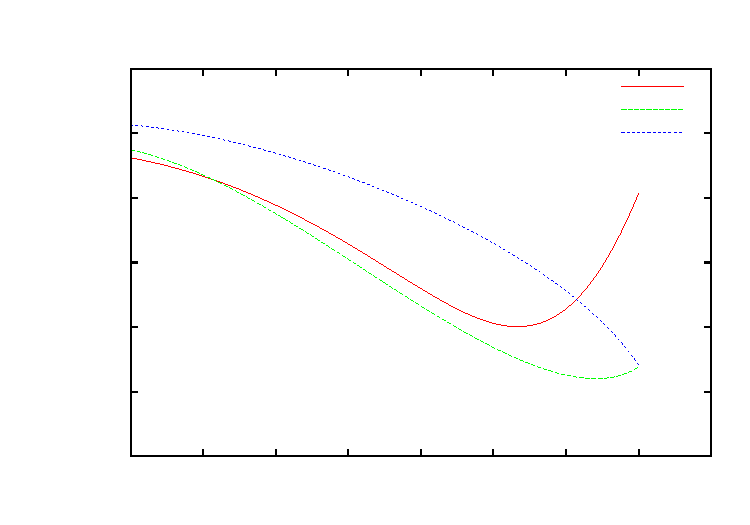
\includegraphics{symmetric_hfl6_2_2}}%
    \gplfronttext
  \end{picture}%
\endgroup

		\caption{First-order corrections to energy per particle, with the orbital angular momentum truncated at 6 and a cutoff $\lambda=2.1$, $\lambda=2.2$ fm$-1$ and $\lambda=2.5$ fm$^{-1}$.}
		\label{fig:hf23}
\end{figure}
\begin{figure}
% GNUPLOT: LaTeX picture with Postscript
\begingroup
  \makeatletter
  \providecommand\color[2][]{%
    \GenericError{(gnuplot) \space\space\space\@spaces}{%
      Package color not loaded in conjunction with
      terminal option `colourtext'%
    }{See the gnuplot documentation for explanation.%
    }{Either use 'blacktext' in gnuplot or load the package
      color.sty in LaTeX.}%
    \renewcommand\color[2][]{}%
  }%
  \providecommand\includegraphics[2][]{%
    \GenericError{(gnuplot) \space\space\space\@spaces}{%
      Package graphicx or graphics not loaded%
    }{See the gnuplot documentation for explanation.%
    }{The gnuplot epslatex terminal needs graphicx.sty or graphics.sty.}%
    \renewcommand\includegraphics[2][]{}%
  }%
  \providecommand\rotatebox[2]{#2}%
  \@ifundefined{ifGPcolor}{%
    \newif\ifGPcolor
    \GPcolortrue
  }{}%
  \@ifundefined{ifGPblacktext}{%
    \newif\ifGPblacktext
    \GPblacktexttrue
  }{}%
  % define a \g@addto@macro without @ in the name:
  \let\gplgaddtomacro\g@addto@macro
  % define empty templates for all commands taking text:
  \gdef\gplbacktext{}%
  \gdef\gplfronttext{}%
  \makeatother
  \ifGPblacktext
    % no textcolor at all
    \def\colorrgb#1{}%
    \def\colorgray#1{}%
  \else
    % gray or color?
    \ifGPcolor
      \def\colorrgb#1{\color[rgb]{#1}}%
      \def\colorgray#1{\color[gray]{#1}}%
      \expandafter\def\csname LTw\endcsname{\color{white}}%
      \expandafter\def\csname LTb\endcsname{\color{black}}%
      \expandafter\def\csname LTa\endcsname{\color{black}}%
      \expandafter\def\csname LT0\endcsname{\color[rgb]{1,0,0}}%
      \expandafter\def\csname LT1\endcsname{\color[rgb]{0,1,0}}%
      \expandafter\def\csname LT2\endcsname{\color[rgb]{0,0,1}}%
      \expandafter\def\csname LT3\endcsname{\color[rgb]{1,0,1}}%
      \expandafter\def\csname LT4\endcsname{\color[rgb]{0,1,1}}%
      \expandafter\def\csname LT5\endcsname{\color[rgb]{1,1,0}}%
      \expandafter\def\csname LT6\endcsname{\color[rgb]{0,0,0}}%
      \expandafter\def\csname LT7\endcsname{\color[rgb]{1,0.3,0}}%
      \expandafter\def\csname LT8\endcsname{\color[rgb]{0.5,0.5,0.5}}%
    \else
      % gray
      \def\colorrgb#1{\color{black}}%
      \def\colorgray#1{\color[gray]{#1}}%
      \expandafter\def\csname LTw\endcsname{\color{white}}%
      \expandafter\def\csname LTb\endcsname{\color{black}}%
      \expandafter\def\csname LTa\endcsname{\color{black}}%
      \expandafter\def\csname LT0\endcsname{\color{black}}%
      \expandafter\def\csname LT1\endcsname{\color{black}}%
      \expandafter\def\csname LT2\endcsname{\color{black}}%
      \expandafter\def\csname LT3\endcsname{\color{black}}%
      \expandafter\def\csname LT4\endcsname{\color{black}}%
      \expandafter\def\csname LT5\endcsname{\color{black}}%
      \expandafter\def\csname LT6\endcsname{\color{black}}%
      \expandafter\def\csname LT7\endcsname{\color{black}}%
      \expandafter\def\csname LT8\endcsname{\color{black}}%
    \fi
  \fi
  \setlength{\unitlength}{0.0500bp}%
  \begin{picture}(7200.00,5040.00)%
    \gplgaddtomacro\gplbacktext{%
      \csname LTb\endcsname%
      \put(990,660){\makebox(0,0)[r]{\strut{}$-5$}}%
      \put(990,1117){\makebox(0,0)[r]{\strut{}$-4$}}%
      \put(990,1575){\makebox(0,0)[r]{\strut{}$-3$}}%
      \put(990,2032){\makebox(0,0)[r]{\strut{}$-2$}}%
      \put(990,2489){\makebox(0,0)[r]{\strut{}$-1$}}%
      \put(990,2947){\makebox(0,0)[r]{\strut{}$0$}}%
      \put(990,3404){\makebox(0,0)[r]{\strut{}$1$}}%
      \put(990,3861){\makebox(0,0)[r]{\strut{}$2$}}%
      \put(990,4319){\makebox(0,0)[r]{\strut{}$3$}}%
      \put(990,4776){\makebox(0,0)[r]{\strut{}$4$}}%
      \put(1122,440){\makebox(0,0){\strut{}$1.2$}}%
      \put(1835,440){\makebox(0,0){\strut{}$1.3$}}%
      \put(2548,440){\makebox(0,0){\strut{}$1.4$}}%
      \put(3261,440){\makebox(0,0){\strut{}$1.5$}}%
      \put(3974,440){\makebox(0,0){\strut{}$1.6$}}%
      \put(4687,440){\makebox(0,0){\strut{}$1.7$}}%
      \put(5400,440){\makebox(0,0){\strut{}$1.8$}}%
      \put(6113,440){\makebox(0,0){\strut{}$1.9$}}%
      \put(6826,440){\makebox(0,0){\strut{}$2$}}%
      \put(220,2718){\rotatebox{90}{\makebox(0,0){\strut{}E/A [MeV]}}}%
      \put(3974,110){\makebox(0,0){\strut{}$k_f$ [fm$^{-1}$]}}%
    }%
    \gplgaddtomacro\gplfronttext{%
      \csname LTb\endcsname%
      \put(6339,4603){\makebox(0,0)[r]{\strut{}E/A for symmetric nuclear matter, l=4 $\lambda=2.1$, fm$^{-1}$}}%
    }%
    \gplbacktext
    \put(0,0){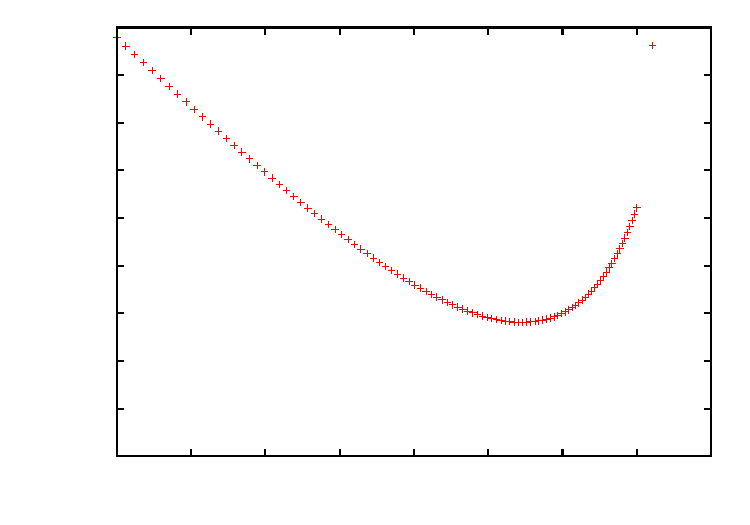
\includegraphics{nuclearmatterl_4_2_1}}%
    \gplfronttext
  \end{picture}%
\endgroup

\caption{Coupled cluster calculations on nuclear matter, with $l=4$ and cutoff $\lambda=2.1$ fm$^{-1}$.}
\label{fig:ccm_nucl_4_21}
\end{figure}
\begin{figure}
% GNUPLOT: LaTeX picture with Postscript
\begingroup
  \makeatletter
  \providecommand\color[2][]{%
    \GenericError{(gnuplot) \space\space\space\@spaces}{%
      Package color not loaded in conjunction with
      terminal option `colourtext'%
    }{See the gnuplot documentation for explanation.%
    }{Either use 'blacktext' in gnuplot or load the package
      color.sty in LaTeX.}%
    \renewcommand\color[2][]{}%
  }%
  \providecommand\includegraphics[2][]{%
    \GenericError{(gnuplot) \space\space\space\@spaces}{%
      Package graphicx or graphics not loaded%
    }{See the gnuplot documentation for explanation.%
    }{The gnuplot epslatex terminal needs graphicx.sty or graphics.sty.}%
    \renewcommand\includegraphics[2][]{}%
  }%
  \providecommand\rotatebox[2]{#2}%
  \@ifundefined{ifGPcolor}{%
    \newif\ifGPcolor
    \GPcolortrue
  }{}%
  \@ifundefined{ifGPblacktext}{%
    \newif\ifGPblacktext
    \GPblacktexttrue
  }{}%
  % define a \g@addto@macro without @ in the name:
  \let\gplgaddtomacro\g@addto@macro
  % define empty templates for all commands taking text:
  \gdef\gplbacktext{}%
  \gdef\gplfronttext{}%
  \makeatother
  \ifGPblacktext
    % no textcolor at all
    \def\colorrgb#1{}%
    \def\colorgray#1{}%
  \else
    % gray or color?
    \ifGPcolor
      \def\colorrgb#1{\color[rgb]{#1}}%
      \def\colorgray#1{\color[gray]{#1}}%
      \expandafter\def\csname LTw\endcsname{\color{white}}%
      \expandafter\def\csname LTb\endcsname{\color{black}}%
      \expandafter\def\csname LTa\endcsname{\color{black}}%
      \expandafter\def\csname LT0\endcsname{\color[rgb]{1,0,0}}%
      \expandafter\def\csname LT1\endcsname{\color[rgb]{0,1,0}}%
      \expandafter\def\csname LT2\endcsname{\color[rgb]{0,0,1}}%
      \expandafter\def\csname LT3\endcsname{\color[rgb]{1,0,1}}%
      \expandafter\def\csname LT4\endcsname{\color[rgb]{0,1,1}}%
      \expandafter\def\csname LT5\endcsname{\color[rgb]{1,1,0}}%
      \expandafter\def\csname LT6\endcsname{\color[rgb]{0,0,0}}%
      \expandafter\def\csname LT7\endcsname{\color[rgb]{1,0.3,0}}%
      \expandafter\def\csname LT8\endcsname{\color[rgb]{0.5,0.5,0.5}}%
    \else
      % gray
      \def\colorrgb#1{\color{black}}%
      \def\colorgray#1{\color[gray]{#1}}%
      \expandafter\def\csname LTw\endcsname{\color{white}}%
      \expandafter\def\csname LTb\endcsname{\color{black}}%
      \expandafter\def\csname LTa\endcsname{\color{black}}%
      \expandafter\def\csname LT0\endcsname{\color{black}}%
      \expandafter\def\csname LT1\endcsname{\color{black}}%
      \expandafter\def\csname LT2\endcsname{\color{black}}%
      \expandafter\def\csname LT3\endcsname{\color{black}}%
      \expandafter\def\csname LT4\endcsname{\color{black}}%
      \expandafter\def\csname LT5\endcsname{\color{black}}%
      \expandafter\def\csname LT6\endcsname{\color{black}}%
      \expandafter\def\csname LT7\endcsname{\color{black}}%
      \expandafter\def\csname LT8\endcsname{\color{black}}%
    \fi
  \fi
  \setlength{\unitlength}{0.0500bp}%
  \begin{picture}(7200.00,5040.00)%
    \gplgaddtomacro\gplbacktext{%
      \csname LTb\endcsname%
      \put(990,660){\makebox(0,0)[r]{\strut{}$10$}}%
      \put(990,1280){\makebox(0,0)[r]{\strut{}$15$}}%
      \put(990,1900){\makebox(0,0)[r]{\strut{}$20$}}%
      \put(990,2520){\makebox(0,0)[r]{\strut{}$25$}}%
      \put(990,3140){\makebox(0,0)[r]{\strut{}$30$}}%
      \put(990,3760){\makebox(0,0)[r]{\strut{}$35$}}%
      \put(990,4380){\makebox(0,0)[r]{\strut{}$40$}}%
      \put(1122,440){\makebox(0,0){\strut{}$1.2$}}%
      \put(1835,440){\makebox(0,0){\strut{}$1.3$}}%
      \put(2548,440){\makebox(0,0){\strut{}$1.4$}}%
      \put(3261,440){\makebox(0,0){\strut{}$1.5$}}%
      \put(3974,440){\makebox(0,0){\strut{}$1.6$}}%
      \put(4687,440){\makebox(0,0){\strut{}$1.7$}}%
      \put(5400,440){\makebox(0,0){\strut{}$1.8$}}%
      \put(6113,440){\makebox(0,0){\strut{}$1.9$}}%
      \put(6826,440){\makebox(0,0){\strut{}$2$}}%
      \put(220,2520){\rotatebox{90}{\makebox(0,0){\strut{}E/A [MeV]}}}%
      \put(3974,110){\makebox(0,0){\strut{}$k_f$}}%
      \put(3974,4710){\makebox(0,0){\strut{}First order energies for pure neutron matter, $l=4$}}%
    }%
    \gplgaddtomacro\gplfronttext{%
      \csname LTb\endcsname%
      \put(5839,4207){\makebox(0,0)[r]{\strut{}$\lambda$=2.1 fm$^{-1}$}}%
      \csname LTb\endcsname%
      \put(5839,3987){\makebox(0,0)[r]{\strut{}$\lambda$=2.2 fm$^{-1}$}}%
      \csname LTb\endcsname%
      \put(5839,3767){\makebox(0,0)[r]{\strut{}$\lambda$=2.5 fm$^{-1}$}}%
    }%
    \gplbacktext
    \put(0,0){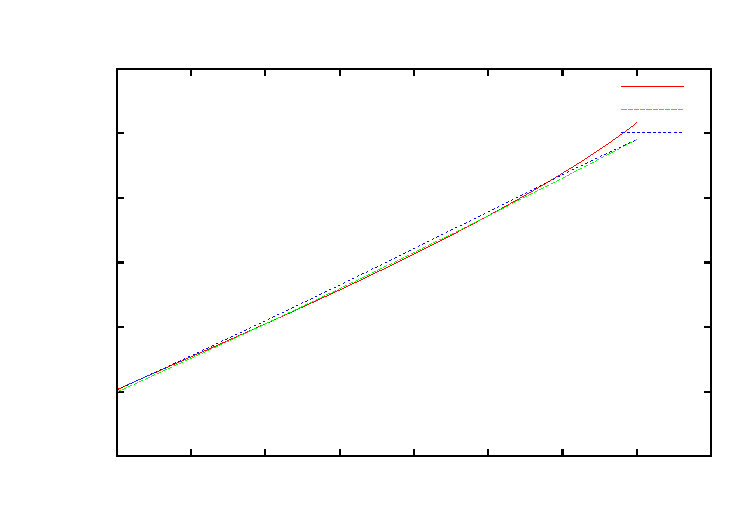
\includegraphics{firstpureneutron_l4}}%
    \gplfronttext
  \end{picture}%
\endgroup

\caption{First order equation of state of pure neutron matter with the cutoff, $\lambda=2.1$ fm$^{-1}$, $\lambda=2.2$~fm$^{-1}$~and $\lambda=2.5$~fm$^{-1}$.}
\label{fig:first_neutron_l4}
\end{figure}
\begin{figure}
% GNUPLOT: LaTeX picture with Postscript
\begingroup
  \makeatletter
  \providecommand\color[2][]{%
    \GenericError{(gnuplot) \space\space\space\@spaces}{%
      Package color not loaded in conjunction with
      terminal option `colourtext'%
    }{See the gnuplot documentation for explanation.%
    }{Either use 'blacktext' in gnuplot or load the package
      color.sty in LaTeX.}%
    \renewcommand\color[2][]{}%
  }%
  \providecommand\includegraphics[2][]{%
    \GenericError{(gnuplot) \space\space\space\@spaces}{%
      Package graphicx or graphics not loaded%
    }{See the gnuplot documentation for explanation.%
    }{The gnuplot epslatex terminal needs graphicx.sty or graphics.sty.}%
    \renewcommand\includegraphics[2][]{}%
  }%
  \providecommand\rotatebox[2]{#2}%
  \@ifundefined{ifGPcolor}{%
    \newif\ifGPcolor
    \GPcolortrue
  }{}%
  \@ifundefined{ifGPblacktext}{%
    \newif\ifGPblacktext
    \GPblacktexttrue
  }{}%
  % define a \g@addto@macro without @ in the name:
  \let\gplgaddtomacro\g@addto@macro
  % define empty templates for all commands taking text:
  \gdef\gplbacktext{}%
  \gdef\gplfronttext{}%
  \makeatother
  \ifGPblacktext
    % no textcolor at all
    \def\colorrgb#1{}%
    \def\colorgray#1{}%
  \else
    % gray or color?
    \ifGPcolor
      \def\colorrgb#1{\color[rgb]{#1}}%
      \def\colorgray#1{\color[gray]{#1}}%
      \expandafter\def\csname LTw\endcsname{\color{white}}%
      \expandafter\def\csname LTb\endcsname{\color{black}}%
      \expandafter\def\csname LTa\endcsname{\color{black}}%
      \expandafter\def\csname LT0\endcsname{\color[rgb]{1,0,0}}%
      \expandafter\def\csname LT1\endcsname{\color[rgb]{0,1,0}}%
      \expandafter\def\csname LT2\endcsname{\color[rgb]{0,0,1}}%
      \expandafter\def\csname LT3\endcsname{\color[rgb]{1,0,1}}%
      \expandafter\def\csname LT4\endcsname{\color[rgb]{0,1,1}}%
      \expandafter\def\csname LT5\endcsname{\color[rgb]{1,1,0}}%
      \expandafter\def\csname LT6\endcsname{\color[rgb]{0,0,0}}%
      \expandafter\def\csname LT7\endcsname{\color[rgb]{1,0.3,0}}%
      \expandafter\def\csname LT8\endcsname{\color[rgb]{0.5,0.5,0.5}}%
    \else
      % gray
      \def\colorrgb#1{\color{black}}%
      \def\colorgray#1{\color[gray]{#1}}%
      \expandafter\def\csname LTw\endcsname{\color{white}}%
      \expandafter\def\csname LTb\endcsname{\color{black}}%
      \expandafter\def\csname LTa\endcsname{\color{black}}%
      \expandafter\def\csname LT0\endcsname{\color{black}}%
      \expandafter\def\csname LT1\endcsname{\color{black}}%
      \expandafter\def\csname LT2\endcsname{\color{black}}%
      \expandafter\def\csname LT3\endcsname{\color{black}}%
      \expandafter\def\csname LT4\endcsname{\color{black}}%
      \expandafter\def\csname LT5\endcsname{\color{black}}%
      \expandafter\def\csname LT6\endcsname{\color{black}}%
      \expandafter\def\csname LT7\endcsname{\color{black}}%
      \expandafter\def\csname LT8\endcsname{\color{black}}%
    \fi
  \fi
  \setlength{\unitlength}{0.0500bp}%
  \begin{picture}(7200.00,5040.00)%
    \gplgaddtomacro\gplbacktext{%
      \csname LTb\endcsname%
      \put(990,660){\makebox(0,0)[r]{\strut{}$12$}}%
      \put(990,1032){\makebox(0,0)[r]{\strut{}$14$}}%
      \put(990,1404){\makebox(0,0)[r]{\strut{}$16$}}%
      \put(990,1776){\makebox(0,0)[r]{\strut{}$18$}}%
      \put(990,2148){\makebox(0,0)[r]{\strut{}$20$}}%
      \put(990,2520){\makebox(0,0)[r]{\strut{}$22$}}%
      \put(990,2892){\makebox(0,0)[r]{\strut{}$24$}}%
      \put(990,3264){\makebox(0,0)[r]{\strut{}$26$}}%
      \put(990,3636){\makebox(0,0)[r]{\strut{}$28$}}%
      \put(990,4008){\makebox(0,0)[r]{\strut{}$30$}}%
      \put(990,4380){\makebox(0,0)[r]{\strut{}$32$}}%
      \put(1122,440){\makebox(0,0){\strut{}$1.2$}}%
      \put(1835,440){\makebox(0,0){\strut{}$1.3$}}%
      \put(2548,440){\makebox(0,0){\strut{}$1.4$}}%
      \put(3261,440){\makebox(0,0){\strut{}$1.5$}}%
      \put(3974,440){\makebox(0,0){\strut{}$1.6$}}%
      \put(4687,440){\makebox(0,0){\strut{}$1.7$}}%
      \put(5400,440){\makebox(0,0){\strut{}$1.8$}}%
      \put(6113,440){\makebox(0,0){\strut{}$1.9$}}%
      \put(6826,440){\makebox(0,0){\strut{}$2$}}%
      \put(220,2520){\rotatebox{90}{\makebox(0,0){\strut{}E/A [MeV]}}}%
      \put(3974,110){\makebox(0,0){\strut{}$k_f$}}%
      \put(3974,4710){\makebox(0,0){\strut{}First order energies for pure neutron matter, $l=6$}}%
    }%
    \gplgaddtomacro\gplfronttext{%
      \csname LTb\endcsname%
      \put(5839,4207){\makebox(0,0)[r]{\strut{}$\lambda$=2.2 fm$^{-1}$}}%
    }%
    \gplbacktext
    \put(0,0){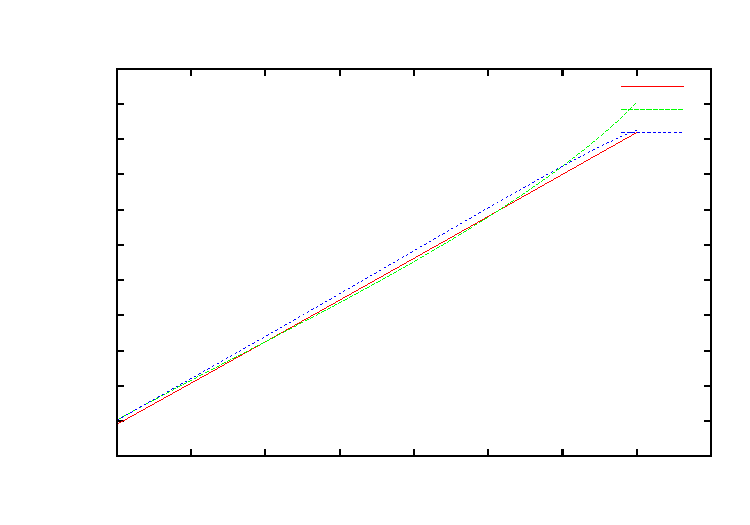
\includegraphics{firstpureneutron_l6}}%
    \gplfronttext
  \end{picture}%
\endgroup

\caption{First order equation of state of pure neutron matter with the cutoff $\lambda=2.1$~fm$^{-1}$, $\lambda=2.2$~and $\lambda=2.5$ fm$^{-1}$. Orbital momentum truncated at 6.}
\label{fig:first_neutron_l6}
\end{figure}
%
\begin{figure}
% GNUPLOT: LaTeX picture with Postscript
\begingroup
  \makeatletter
  \providecommand\color[2][]{%
    \GenericError{(gnuplot) \space\space\space\@spaces}{%
      Package color not loaded in conjunction with
      terminal option `colourtext'%
    }{See the gnuplot documentation for explanation.%
    }{Either use 'blacktext' in gnuplot or load the package
      color.sty in LaTeX.}%
    \renewcommand\color[2][]{}%
  }%
  \providecommand\includegraphics[2][]{%
    \GenericError{(gnuplot) \space\space\space\@spaces}{%
      Package graphicx or graphics not loaded%
    }{See the gnuplot documentation for explanation.%
    }{The gnuplot epslatex terminal needs graphicx.sty or graphics.sty.}%
    \renewcommand\includegraphics[2][]{}%
  }%
  \providecommand\rotatebox[2]{#2}%
  \@ifundefined{ifGPcolor}{%
    \newif\ifGPcolor
    \GPcolortrue
  }{}%
  \@ifundefined{ifGPblacktext}{%
    \newif\ifGPblacktext
    \GPblacktexttrue
  }{}%
  % define a \g@addto@macro without @ in the name:
  \let\gplgaddtomacro\g@addto@macro
  % define empty templates for all commands taking text:
  \gdef\gplbacktext{}%
  \gdef\gplfronttext{}%
  \makeatother
  \ifGPblacktext
    % no textcolor at all
    \def\colorrgb#1{}%
    \def\colorgray#1{}%
  \else
    % gray or color?
    \ifGPcolor
      \def\colorrgb#1{\color[rgb]{#1}}%
      \def\colorgray#1{\color[gray]{#1}}%
      \expandafter\def\csname LTw\endcsname{\color{white}}%
      \expandafter\def\csname LTb\endcsname{\color{black}}%
      \expandafter\def\csname LTa\endcsname{\color{black}}%
      \expandafter\def\csname LT0\endcsname{\color[rgb]{1,0,0}}%
      \expandafter\def\csname LT1\endcsname{\color[rgb]{0,1,0}}%
      \expandafter\def\csname LT2\endcsname{\color[rgb]{0,0,1}}%
      \expandafter\def\csname LT3\endcsname{\color[rgb]{1,0,1}}%
      \expandafter\def\csname LT4\endcsname{\color[rgb]{0,1,1}}%
      \expandafter\def\csname LT5\endcsname{\color[rgb]{1,1,0}}%
      \expandafter\def\csname LT6\endcsname{\color[rgb]{0,0,0}}%
      \expandafter\def\csname LT7\endcsname{\color[rgb]{1,0.3,0}}%
      \expandafter\def\csname LT8\endcsname{\color[rgb]{0.5,0.5,0.5}}%
    \else
      % gray
      \def\colorrgb#1{\color{black}}%
      \def\colorgray#1{\color[gray]{#1}}%
      \expandafter\def\csname LTw\endcsname{\color{white}}%
      \expandafter\def\csname LTb\endcsname{\color{black}}%
      \expandafter\def\csname LTa\endcsname{\color{black}}%
      \expandafter\def\csname LT0\endcsname{\color{black}}%
      \expandafter\def\csname LT1\endcsname{\color{black}}%
      \expandafter\def\csname LT2\endcsname{\color{black}}%
      \expandafter\def\csname LT3\endcsname{\color{black}}%
      \expandafter\def\csname LT4\endcsname{\color{black}}%
      \expandafter\def\csname LT5\endcsname{\color{black}}%
      \expandafter\def\csname LT6\endcsname{\color{black}}%
      \expandafter\def\csname LT7\endcsname{\color{black}}%
      \expandafter\def\csname LT8\endcsname{\color{black}}%
    \fi
  \fi
  \setlength{\unitlength}{0.0500bp}%
  \begin{picture}(7200.00,5040.00)%
    \gplgaddtomacro\gplbacktext{%
      \csname LTb\endcsname%
      \put(990,440){\makebox(0,0)[r]{\strut{}$10$}}%
      \put(990,1097){\makebox(0,0)[r]{\strut{}$15$}}%
      \put(990,1753){\makebox(0,0)[r]{\strut{}$20$}}%
      \put(990,2410){\makebox(0,0)[r]{\strut{}$25$}}%
      \put(990,3067){\makebox(0,0)[r]{\strut{}$30$}}%
      \put(990,3723){\makebox(0,0)[r]{\strut{}$35$}}%
      \put(990,4380){\makebox(0,0)[r]{\strut{}$40$}}%
      \put(1122,220){\makebox(0,0){\strut{}$1.2$}}%
      \put(1835,220){\makebox(0,0){\strut{}$1.3$}}%
      \put(2548,220){\makebox(0,0){\strut{}$1.4$}}%
      \put(3261,220){\makebox(0,0){\strut{}$1.5$}}%
      \put(3974,220){\makebox(0,0){\strut{}$1.6$}}%
      \put(4687,220){\makebox(0,0){\strut{}$1.7$}}%
      \put(5400,220){\makebox(0,0){\strut{}$1.8$}}%
      \put(6113,220){\makebox(0,0){\strut{}$1.9$}}%
      \put(6826,220){\makebox(0,0){\strut{}$2$}}%
      \put(220,2410){\rotatebox{90}{\makebox(0,0){\strut{}E/A [MeV]}}}%
      \put(3974,4710){\makebox(0,0){\strut{}Coupled cluster energies for pure neutron matter, $l=4$.}}%
    }%
    \gplgaddtomacro\gplfronttext{%
      \csname LTb\endcsname%
      \put(5839,4207){\makebox(0,0)[r]{\strut{}$\lambda=2.1$ fm$^{-1}$}}%
      \csname LTb\endcsname%
      \put(5839,3987){\makebox(0,0)[r]{\strut{}$\lambda=2.2$ fm$^{-1}$}}%
    }%
    \gplbacktext
    \put(0,0){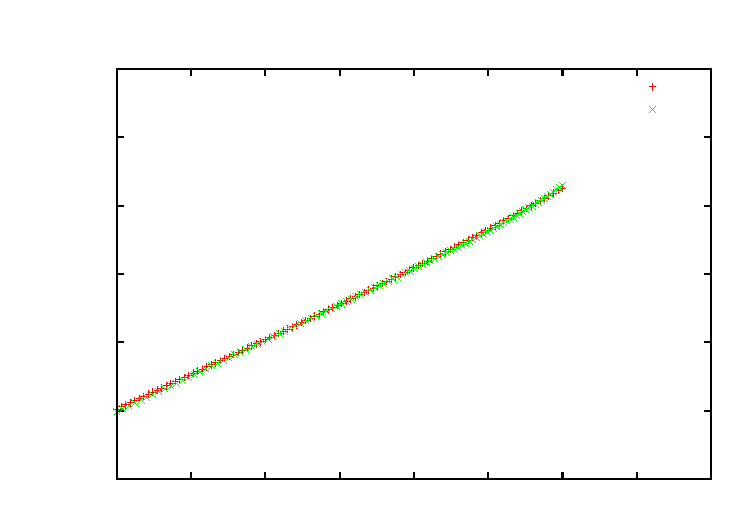
\includegraphics{neutronmatterl_4}}%
    \gplfronttext
  \end{picture}%
\endgroup

\caption{Coupled cluster calculations on pure neutron matter with the cutoff on momentum at $\lambda=2.1$ fm$^{-1}$ and orbital angular momentum $l=4$.}
\label{fig:ccm_net_4_21}
\end{figure}



\subsection{Conclusion}

We can affirm that it is possible to perform coupled cluster calculations on 
nuclear matter, we have seen an explicit convergence at least for the cutoff 
$\lambda=2.1$ fm$^{-1}$. For the cases without convergence as for 
$k_f=1.8$ fm$^{-1}$ with $\lambda=2.2$ fm$^{-1}$, $\lambda=2.5$ fm$^{-1}$ and 
$\lambda=3.0$ fm$^{-1}$ may be as a consequence of the primitive linear iteration scheme.  
As expected the convergence is faster for a smaller cutoff. This, because 
with a larger cutoff we expect more contributions from intermediate states which
we can see from table \ref{tab:korreksjoner}. The model space is smaller and we have fewer particle states with small cutoffs.
However we must admit that some of the results were not as expected, the corrections to the
first-order energy was expected to be higher, and we also notice that it seems
that the first-order energy blows up by including more orbital angular
momenta in the laboratory system. \\
\\
From Fig. \ref{fig:hf21} we see that the energy density is highly dependent on 
the cutoff and we do not think it is fair to favor one cutoff over another, even if a cutoff reproduces the experimental value. %it is not
%fair to state that one cutoff is more correct than another. 
It may seem 
that we need a better understanding of the nuclear interactions. In Ref.
\cite{inmedium} they claim that most of the theoretical calculations on the binding energy of nuclear
matter  overbind the system up to 25\%, however some calculations also underbind
the system, which may indicate a lack of understanding the nucleon-nucleon interactions.
We also observe that the corrections to the energy is higher for a larger cutoff
$\lambda$ which indicates that the intermediate states contribute more. 
We ''lose'' physics when the cutoff is lowered.\\ 
\\
As an improvement to the project and the
calculations could be to include relativistic effects and three-body forces 
which are believed to be necessary in nuclear matter calculations. It could be 
convenient to make the coupled cluster program more efficient. The interaction 
files are huge and require much memory when the program stores the interactions
in arrays.   
